\documentclass[final, hyperref, table]{beamer}
\mode<presentation>


 %\usepackage[english]{babel} % "babel.sty"
% \usepackage{french}                  % "french.sty"
%  \usepackage{franglais}               % "franglais.sty" (a defaut)
  \usepackage{times}			% ajout times le 30 mai 2003
 
%% --------------------------------------------------------------
%% CODAGE DE POLICES ?
%% Si votre moteur Latex est francise, il est conseille
%% d'utiliser le codage de police T1 pour faciliter la césure,
%% si vous disposez de ces polices (DC/EC)
\usepackage[utf8]{inputenc}
\usepackage[T1]{fontenc}


%% ==============================================================
%\usepackage{graphicx}
\usepackage{amsmath,amsfonts}
%\usepackage[table]{xcolor}
\usepackage{subfigure}
\usepackage{fancybox}
\usepackage{multicol}
\usepackage{wrapfig}
\usepackage{listings}
\usepackage{xcolor}

%\usetheme{Warsaw}
\usetheme{Frankfurt}
%\usetheme{JuanLesPins}
\setbeamercovered{transparent}


% telemeta red
\definecolor{telemetaRed}{rgb}{0.41568, 0.01176, 0.02745}	% #6A0307
\usecolortheme[rgb={0.41568, 0.01176, 0.02745}]{structure} 

\hypersetup{colorlinks, urlcolor=blue, linkcolor=}
% Display a grid to help align images
%\beamertemplategridbackground[1cm]

%We will get the normal bibliography style (number or text instead of icon) by including the following code
\setbeamertemplate{bibliography item}[text]
\setbeamerfont{caption}{size=\footnotesize}
% listings settings
\definecolor{lstComments}{rgb}{0,0.6,0}
\definecolor{lstBkgrd}{rgb}{1,1,0.8}
\lstset{%
  language=Python, % the language of the code
  frame=single,  % adds a frame around the code
  commentstyle=\color{lstComments},% comment style
  backgroundcolor=\color{lstBkgrd},   % choose the background color
  basicstyle=\scriptsize,       % the size of the fonts that are used for the code
  keywordstyle=\color{blue},      % keyword style
  showstringspaces=false,          % underline spaces within strings only
}
\title[Analyse et édition collaboratives des données multimédia]{}%\raisebox{2\height}{\includegraphics[width=0.4\textwidth]{img/logo_telemeta_1-1.pdf}}
\subtitle{Analyse et édition collaboratives des données multimédia}
\author[Guillaume et al.]{\tiny \underline{Guillaume Pellerin\inst{1}}, Thomas Fillon\inst{1,2}, Joséphine Simonnot\inst{3}, Aude Da-Cruz Lima\inst{3}, Marie-France Mifune\inst{4}, Stéphanie Khoury\inst{3}, Maxime Le Coz\inst{5}, Estelle Amy de La Bretèque\inst{3}, David Doukhan\inst{7}, Dominique Fourer\inst{6}, Jean-Luc Rouas\inst{6}, Julien Pinquier\inst{5}, Julie Mauclair\inst{5}, Claude Barras \inst{7}}


\institute[Parisson]{\tiny
  \inst{1}%
  Parisson, Paris, France\\
  \inst{2}%
  LAM, Institut Jean Le Rond d'Alembert, UPMC Univ. Paris 06, UMR CNRS 7190, Paris, France\\
  \inst{3}%
  CREM, LESC, UMR CNRS 7186, MAE, Université Paris Ouest Nanterre La Défense, Nanterre, France\\
  \inst{4}%
  CNRS-MNHN-Université Paris Diderot-Sorbonne Cité, UMR 7206, Paris, France\\
  \inst{5}%
  IRIT - Université Toulouse 3 Paul Sabatier - Toulouse, France\\
  \inst{6}%
  LaBRI - CNRS UMR 5800, Université Bordeaux 1, Talence, France\\
  \inst{7}%
  Université Paris-Sud / CNRS-LIMSI - Orsay, France\\
  %Thanks
 {\tiny \textcolor{red}{\emph{This work was partially done inside the DIADEMS project\\ funded by the French National Research Agency ANR (CONTINT)}}}
}
% \begin{center}
% \hfill
%    \raisebox{-4ex}{
\includegraphics[width=0.1\linewidth]{../poster/img/logo_CREM.png}} \hfill
%   
\includegraphics[width=0.15\linewidth]{img/logo_LESC.png}\hfill
%    \includegraphics[width=.3\linewidth]{img/parisson_logo_FINALE_com.pdf}\hfill
%    \includegraphics[width=.18\linewidth]{img/upmc.png}\hfill
%  \end{center}
\date{{\scriptsize Journée d’étude "La visualisation des données 
numériques"}  
% \raisebox{-0.5\height}{
\includegraphics[width=0.2\textwidth]{dlfm.png}}\\
\footnotesize - 26 septembre 2014 - IRCAM, Paris}
        

\newcommand{\CREM}{Research Center for Ethnomusicology}
\setbeamertemplate{section page}
{
    \begin{centering}
    \begin{beamercolorbox}[sep=12pt,center,rounded=true, shadow=true]{part title}
    \usebeamerfont{section title}\insertsection\par
    \end{beamercolorbox}
    \end{centering}
\tableofcontents[currentsection, hideothersubsections]
}
\AtBeginSection[]{\frame{\sectionpage}}
% \AtBeginSection[] % Do nothing for \section*
% {
% \begin{frame}
% \frametitle{Outline}
% \tableofcontents[currentsection]
% \end{frame}
% }
\begin{document}%\footnotesize
\begin{frame}[plain]
  \begin{center}
    \raisebox{-1cm}{\includegraphics[width=0.4\textwidth]{img/logo_telemeta_1-1.pdf}}
  \end{center}
  \maketitle
\end{frame}

% \begin{frame}\frametitle{Outline}
%   \tableofcontents[hideallsubsections]
% \end{frame}


\section[Introduction]{Introduction}

\subsection{Les besoins}
\begin{frame}\frametitle{Besoins}

   \begin{itemize}
   \item \alert{éditer} les données multimédia et leurs métadonnées, 
   \item \alert{collaborer} à plusieurs niveaux autour d'une même plateforme
   \item \alert{respecter} les droits d'auteurs, d'édition et de publications
   \item \alert{s'affranchir} des formats numériques d'origine
   \item \alert{extrapôler} les modèles de métadonnées dans le temps
   \item \alert{associer} des outils de traitement du signal
   \item \alert{indexer} temporellement les événements 
   \item \alert{pérenniser} les archives ET le système de publication
   \item \alert{passer} l'échelle
   \end{itemize}
\end{frame}

\subsection{Les enjeux}
\begin{frame}\frametitle{Enjeux}

\begin{block}{Les domaines scientifiques}
   \begin{itemize}
   \item Sciences humaines
   \item Sciences de l'information
   \item Sciences physiques
   \item Applications : recherche, enseignement, communication, culture, humanités numériques
   \end{itemize}
\end{block}

\begin{block}{Les moyens}
   \begin{itemize}
   \item Standards du web
   \item Frameworks, workflows, logiciels libres
   \item Données !
   \item Langages !!
   \item Humains !!!
   \end{itemize}
\end{block}

\end{frame}


\section[Telemeta]{La plateforme Telemeta}\label{sec:Telemeta}

\subsection{Le projet Telemeta}
\begin{frame}\frametitle{Le projet Telemeta}
  \begin{block}{Un système de gestion audio web ouvert}
      \begin{itemize}
      \item Développée depuis 2007 (CREM, Parisson)
      \item Disponible depuis 2011
       \vspace{-0.1cm}
       \item Archives sonores du CNRS - Musée de l'Homme
       \begin{center}
        \bf\href{http://archives.crem-cnrs.fr}{archives.crem-cnrs.fr}
       \end{center}
    \item Plateforme collaborative mixant la musicologie, l'anthropologie, la linguistique, l'acoustique, l'informatique
    \end{itemize}   
     
\end{block}

    \begin{block}{Un logiciel libre et open-source}
    \begin{itemize}
    \item Telemeta, is a \alert{free and open source software} (\emph{GPL-like} licence)
       in accordance with \alert{open web standards}.
    \end{itemize}
    \vspace{-0.5cm}
    \begin{center}
      \raisebox{-0.4\height}{\includegraphics[width=0.3\textwidth]{img/logo_telemeta_800.png}}
\hspace{1cm}
      \textbf{\href{http://telemeta.org}{telemeta.org}}
    \end{center}
  \end{block}
\end{frame}


\subsection{Fonctionnalités}
\begin{frame}[label=telemeta_features]{Fonctionnalités}
    \begin{itemize}
      \item \alert{Edition collaborative} à travers des sons, des modèles de métadonnées, des ontologies, des médias associés
      \item \alert{Standardisation} des formats d'échange
      \item \alert{Analyse} audio, \alert{visualisation}, \alert{transcodage} et \alert{encapsulation des métadonnées} à la volée et à la demande
      \item \alert{Annotation et segmentation} humaine ou semi-automatique
      \item \alert{Gestion des utilisateurs}: bureau individuel, listes de lecture, profils et droits d'accès par groupes
      \item \alert{Moteur de recherche}: \hyperlink{geonavigator}{géo-localisation}, instruments, groupes ethniques, etc
      \item \hyperlink{telemeta_languages}{\alert{Support multi-langues}}: actuellement anglais, français, allemand et chinois
      \item \alert{Compatibilité} aux systèmes de moissonnage institutionnels 
      \item Interface utilisateur \alert{100\% HTML5}.
      \end{itemize}
\end{frame}


\begin{frame}[label=telemeta_metadata]{Métadonnées}
\begin{block}{Informations contextuelles (éthnomusicologie)}
  \begin{itemize}
  \item géographiques
  \item culturelles (population, éthnies, langues, ...)
  \item musicales (formations, instruments, ...)
  \item archivistiques (format des supports originaux, dépositaires, collecteurs, ...)
  \end{itemize}
\end{block}

\begin{block}{Données additionelles}
  \begin{itemize}
  \item iconographies (photos, scans, vidéos, notes, ...),
  \item hyperliens
  \item notes
  \end{itemize}
\end{block}
\hyperlink{metadata_example}{\beamerbutton{Examples}    }
\end{frame}


% \begin{frame}{Metadata}{Descriptive and analytical information on the audio content}
% The second type of metadata consists of information about the \alert{audio content} itself. This metadata can provide information about the global content of the audio item or provide \alert{temporally-indexed information}. 
% Such information can be produced eithe
% r:
% \begin{itemize}
% \item by a human expert or
% \item by an automatic computational audio analysis.
% \end{itemize}
% And it can consist either in:
% \begin{itemize}
% \item Visual representation and segmentation or
% \item Annotations
% \end{itemize}

\subsection{Architecture}
\begin{frame}\frametitle{Architecture}
  \begin{center}
    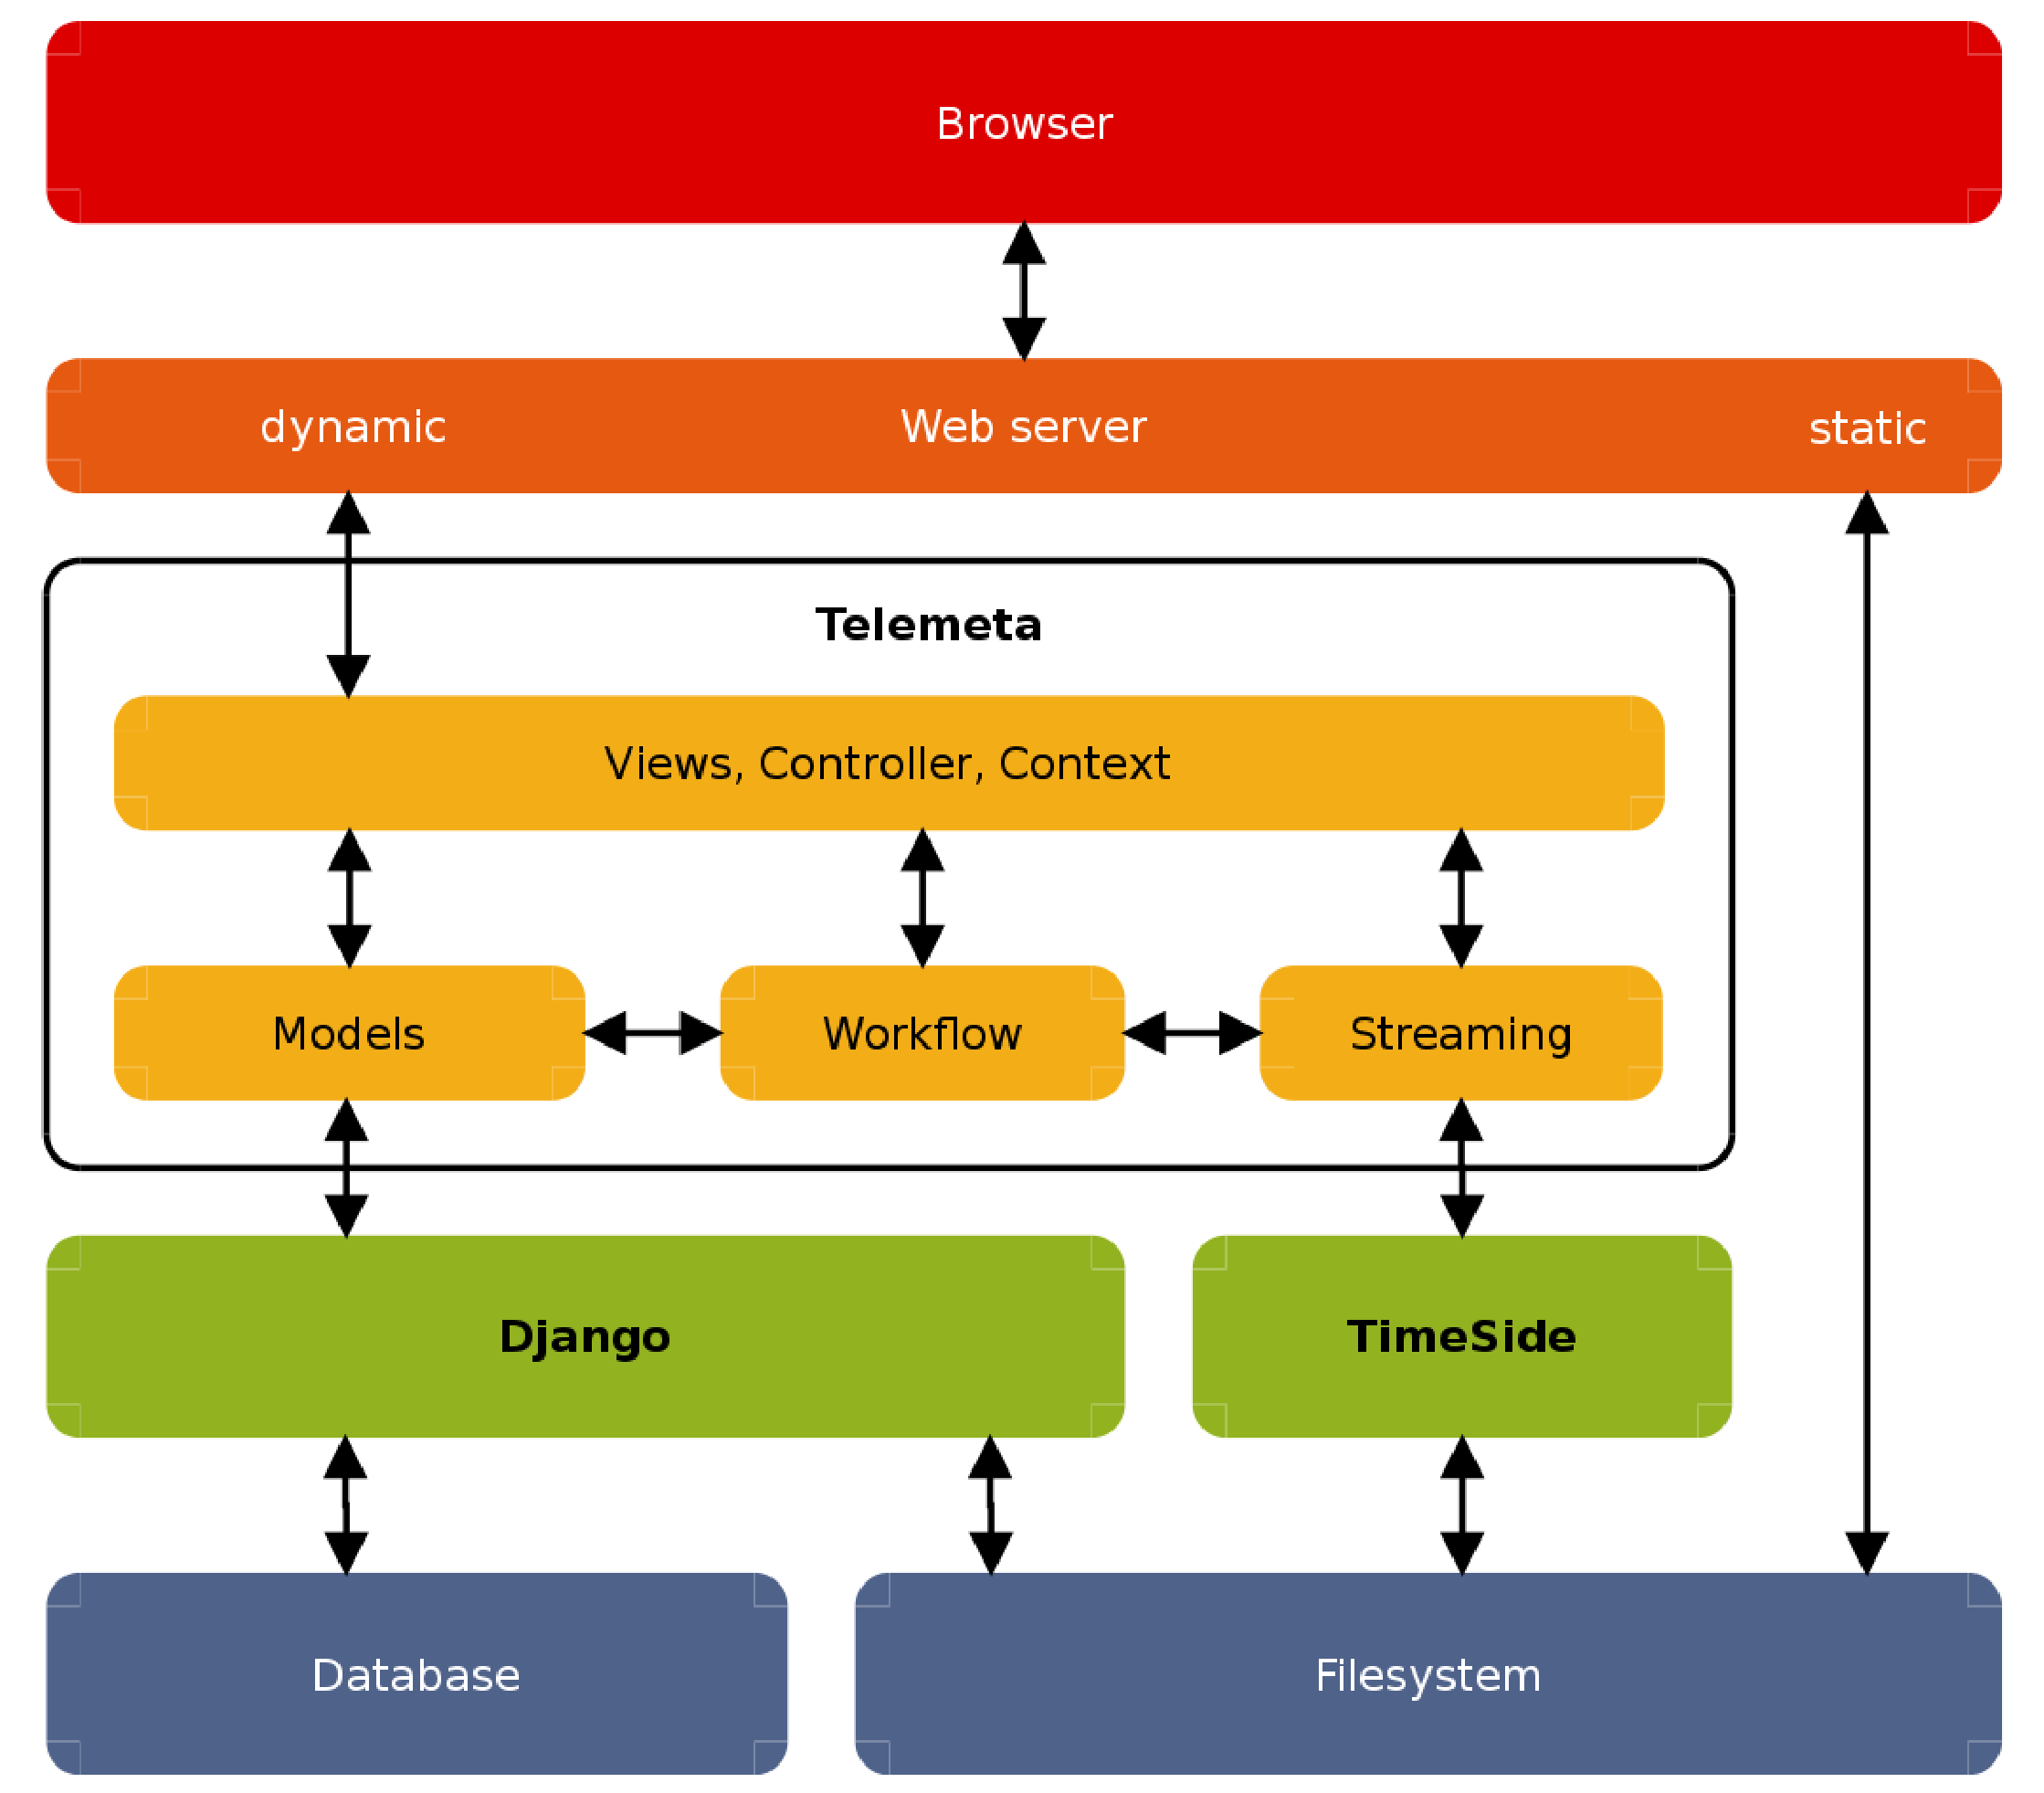
\includegraphics[width=0.75\textwidth]{img/TM_arch.pdf}
  \end{center}
\end{frame}


\subsection{Standards et outils}
\begin{frame}{Standards et outils}
  \begin{block}{Langages, systèmes et formats ouverts}
    \begin{itemize}
    \item WAV, FLAC, OGG, Opus, WebM
    \item HTML, CSS, JavaScript, JSON
    \item DublinCore, OAI-PMH, RDF
    \item Django, TimeSide
    \item Python, C, C++
    \item MySQL, PostgreSQL, MongoDB
    \item GNU, Linux, Docker, Git
    \end{itemize}
    \end{block}

  \begin{block}{Sauvegarde / synchro}%{Content}
    \begin{itemize}
    \item Django (manage.py backup)
    \item RSync + SSH
    \item IRODS
    \end{itemize}
  \end{block}

\end{frame}


\begin{frame}[plain]{Telemeta \emph{Item} page}
  \begin{center}
    \fbox{\includegraphics[width=\linewidth]{img/telemeta_screenshot_en_2.png}}
  \end{center}

\end{frame}

  
% \end{frame}
\begin{frame}{Descriptive and analytical information}
{Visual representation and segmentation}
\scriptsize
\begin{columns}[T]
    \begin{column}{0.6\textwidth}
      \begin{block}{Visual representation of the sound}
       The embedded \alert{TimeSide} audio player allows for a selection
        of various visual representations of the sound (e.g. \alert{waveforms
        and spectrograms}) and some representations of computational
        \alert{analysis}.
      \end{block}
    \end{column}
    \begin{column}{0.3\textwidth}
      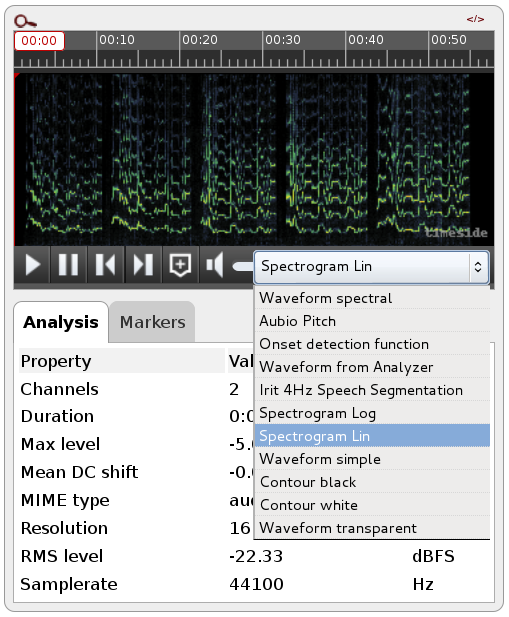
\includegraphics[width=\linewidth]{img/sound_representation.png}
    \end{column}
  \end{columns}
\vspace{-1.5cm}
  \begin{columns}[T]
    \begin{column}{0.6\textwidth}
   \begin{block}<2>{Segmentation}
        Automatic analysis can produce a list of \alert{time-segments}
        associated with \alert{labels} (e.g. detection of spoken versus
        singing voices, chorus, musical instrument categories, and so
        on).
\end{block}
    \end{column}
    \begin{column}{0.3\textwidth} 
  %Detection of spoken voices in a song
    \end{column}
  \end{columns}
  \begin{center}
    \includegraphics<2>[width=0.65\linewidth]{img/IRIT_Speech4Hz.png}
  \end{center}

  
\end{frame}
\begin{frame}{Descriptive and analytical information on the audio content}{Annotations}%\scriptsize
  \begin{columns}[T]
    \begin{column}{0.6\textwidth}
      \begin{block}{Markers}%\tiny
        \begin{itemize}
        \item The embedded audio player also enables annotation of the
          audio content through \alert{time-coded markers}.
        \item These annotations are \alert{indexed through the database}.

        \item Users can create their own annotations and \alert{share} them with colleagues.
   
          % \item \emph{The possibility for experts to annotate
          %   time-segments
          %   over a zoomable representation of the sound is currently
          %   under development in order to improve the accuracy and
          %   the
          %   quality of time-segment-based annotations.}
        \end{itemize}

      \end{block}
    \end{column}

    \begin{column}{0.4\textwidth}
      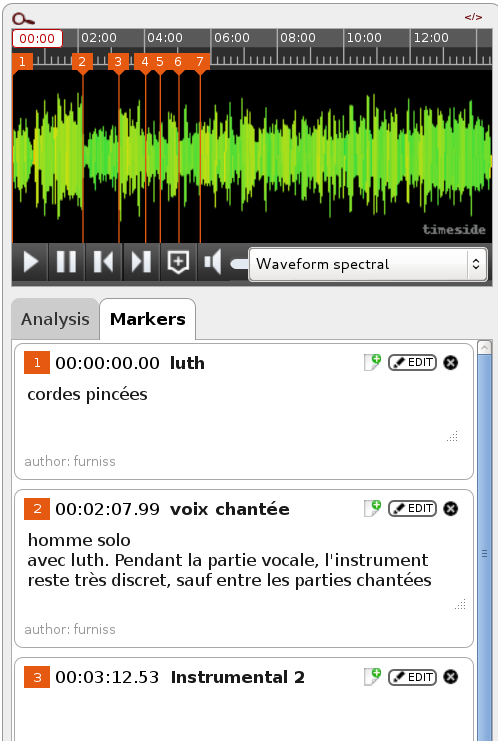
\includegraphics[width=\linewidth]{img/markers.png}
    \end{column}
  \end{columns}
\end{frame}

\section[TimeSide]{Le moteur TimeSide}\label{sec:TimeSide}

\subsection{Goals}
\begin{frame}
 \frametitle{Goals}%\scriptsize
\begin{block}{Server side - TimeSide Engine}
  \begin{itemize}
  \footnotesize
  \item \alert{Do} asynchronous and fast audio processing with Python,
  \item \alert{Decode} audio frames from ANY format into numpy arrays,
  \item \alert{Analyze} audio content with state-of-the-art audio feature extraction libraries (Aubio, Yaafe, Vamp (experimental),
  \item  \alert{Organize}, serialize and save analysis metadata through various formats,
  \item  \alert{Draw} various fancy waveforms, spectrograms and other cool graphers,
  \item  \alert{Transcode} audio data in various media formats and stream them through web apps,
  \end{itemize}
 
\end{block}
\begin{block}{Client side - TimeSide UI}
  \begin{itemize}
  \footnotesize
  \item   \alert{Playback} and  \alert{interact} on demand through a smart high-level HTML5 extensible player,
  \item   \alert{Index},  \alert{tag} and  \alert{organize semantic metadata} \\
(see \href{http://telemeta.org/}{Telemeta} which embeds TimeSide).
  \end{itemize}
\end{block}
\end{frame} 



\subsection{Extraction de features audio}
\begin{frame}{Audio features extraction}
\begin{block}{Audio features extraction}
Embedding state-of-the-art audio feature extraction libraries such as:

\begin{itemize}\footnotesize
\item Aubio:
    \url{http://aubio.org}

\item Yaafe:
    \url{http://yaafe.sourceforge.net}

\item Vamp plugins:  
    \url{http://www.vamp-plugins.org}
\end{itemize}


The results of this
  analysis can be:
  \begin{itemize}\footnotesize
 \item Serialized to the web browser through common markup languages:
    XML, JSON and YAML
  \item Stored in a scientific file format (e.g. NumPy format or
    HDF5)
  \item Exported to sound visualization and annotation software
    (e.g. Sonic Visualizer)
 
  \end{itemize}
\end{block}

\end{frame}
\begin{frame}{TimeSide engine architecture}
  \begin{figure}[htbp]
  \centering
  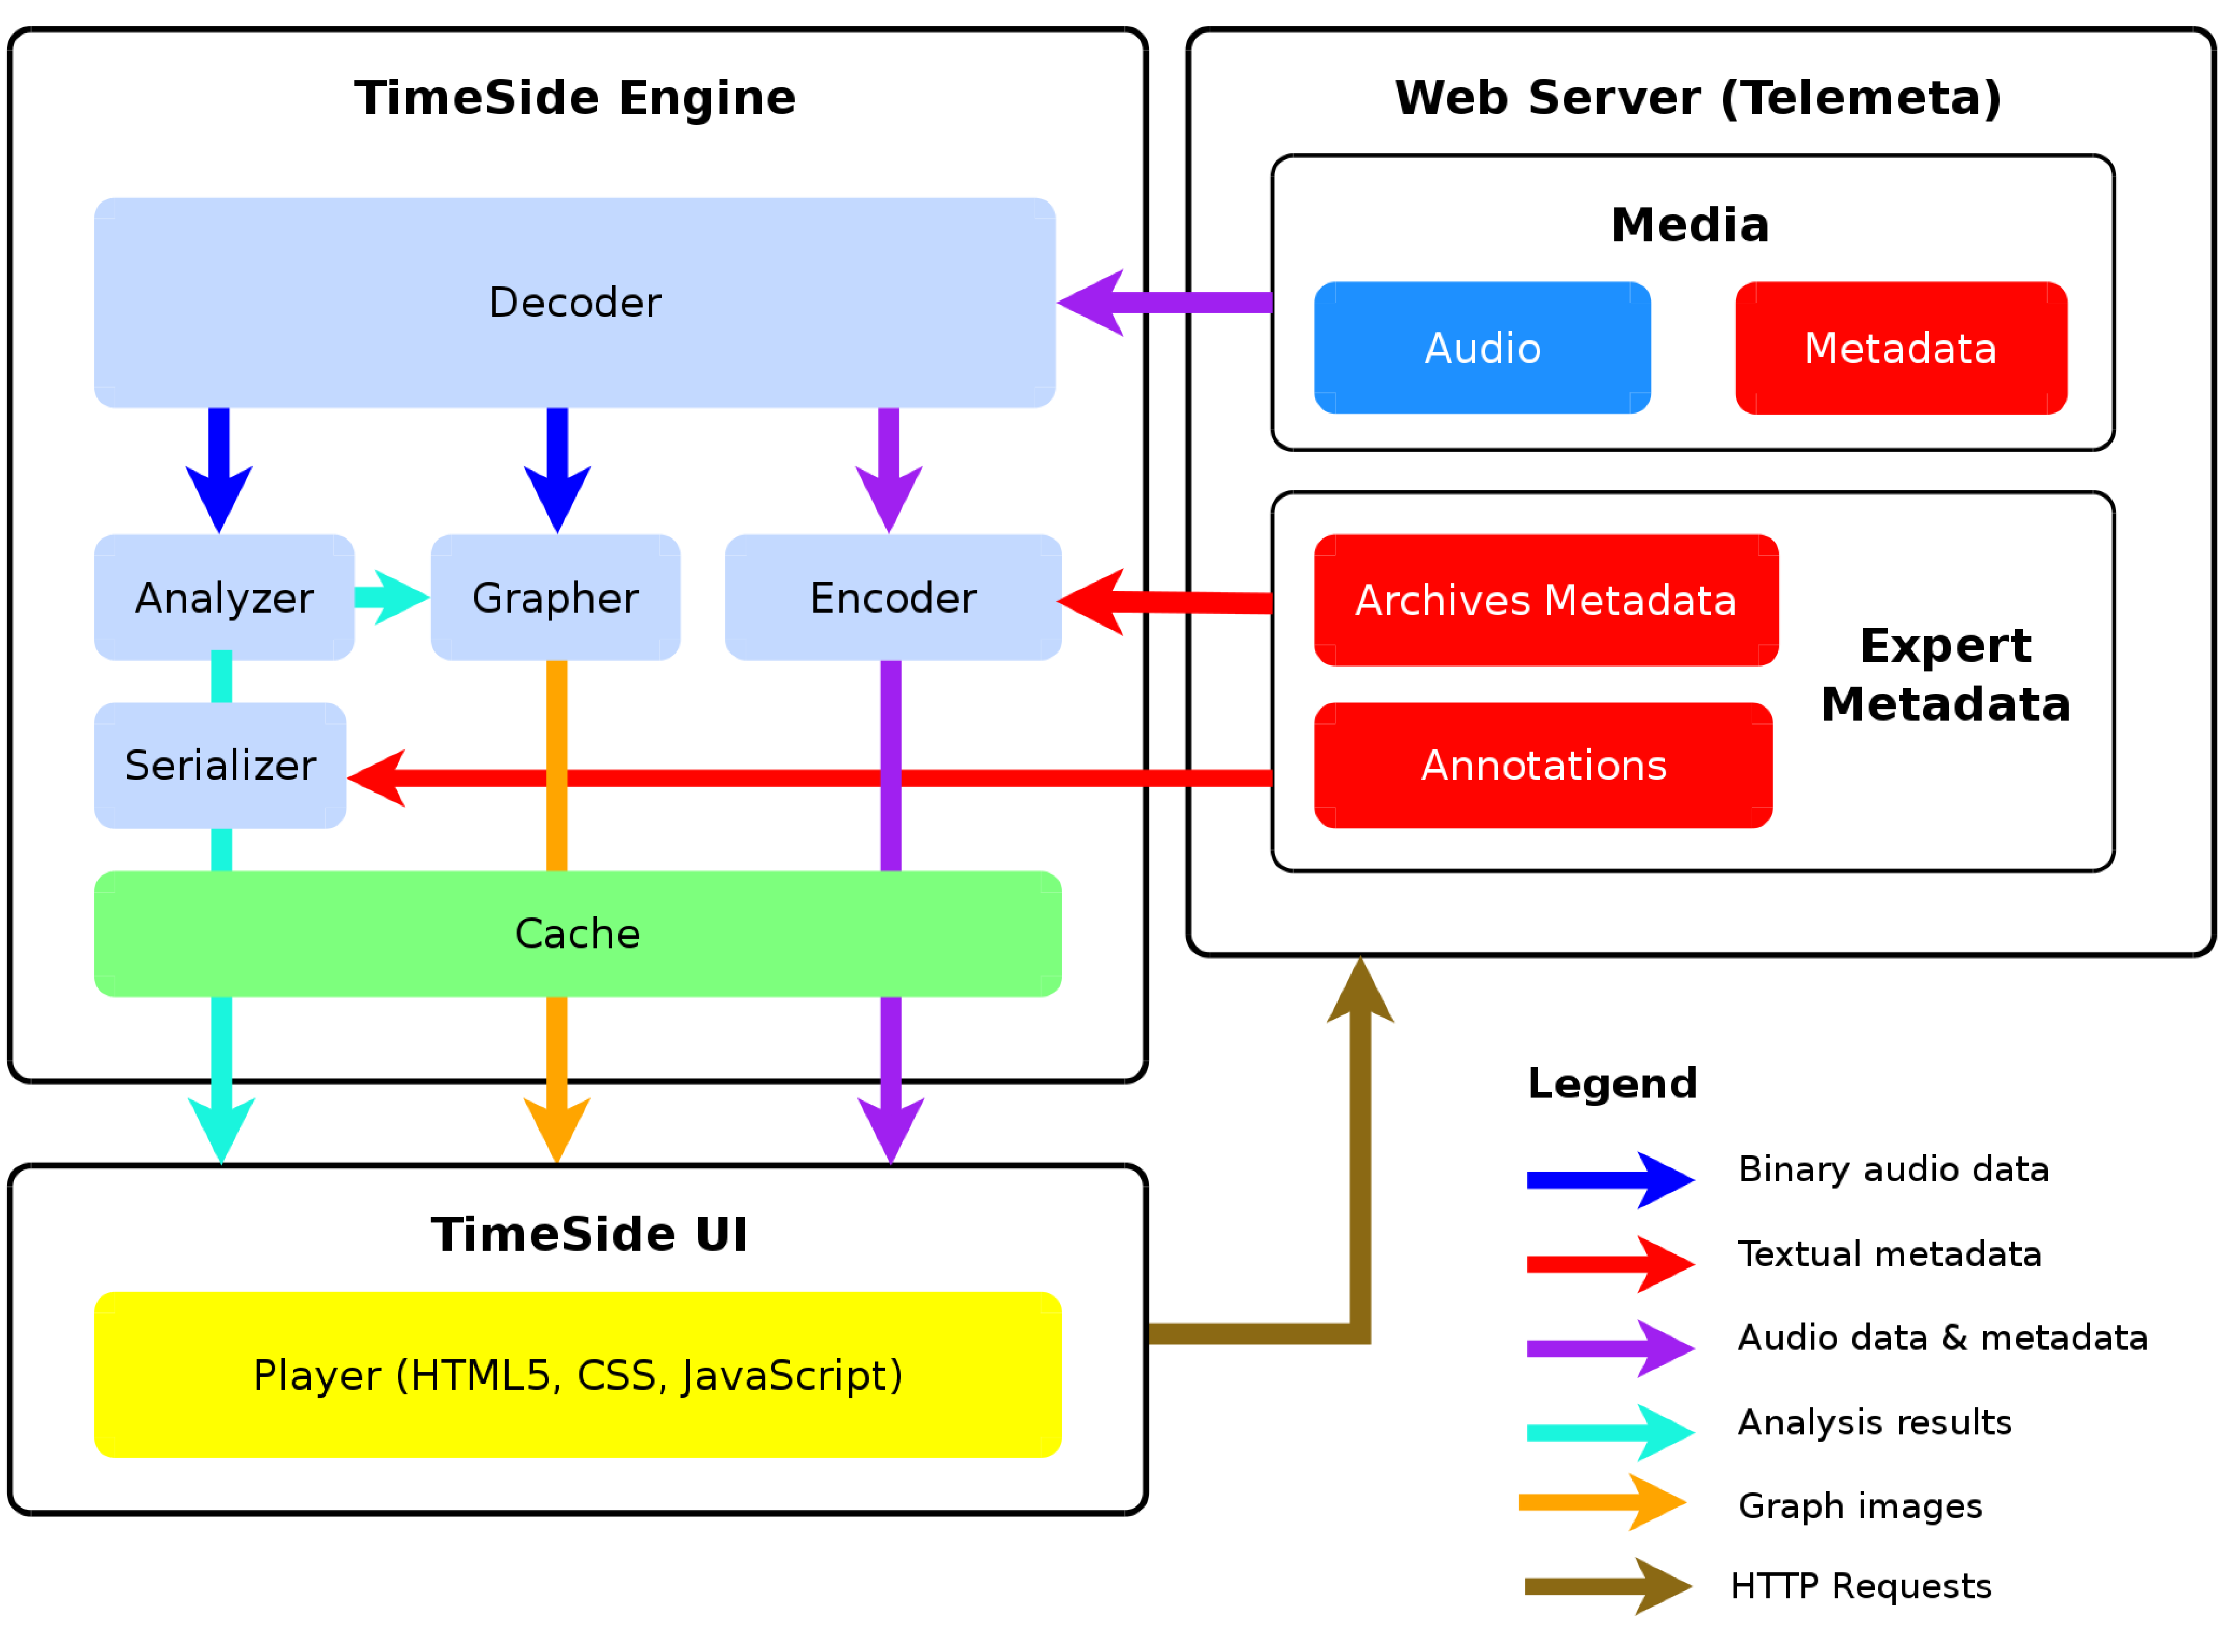
\includegraphics[width=0.8\linewidth]{img/timeside_schema_v3.pdf}
  \caption{TimeSide engine architecture and data flow with Telemeta web-server}\label{fig:TimeSide_Archi}
\end{figure}
\end{frame}
  
\begin{frame}
  \frametitle{TimeSide engine architecture}
  \begin{center}
    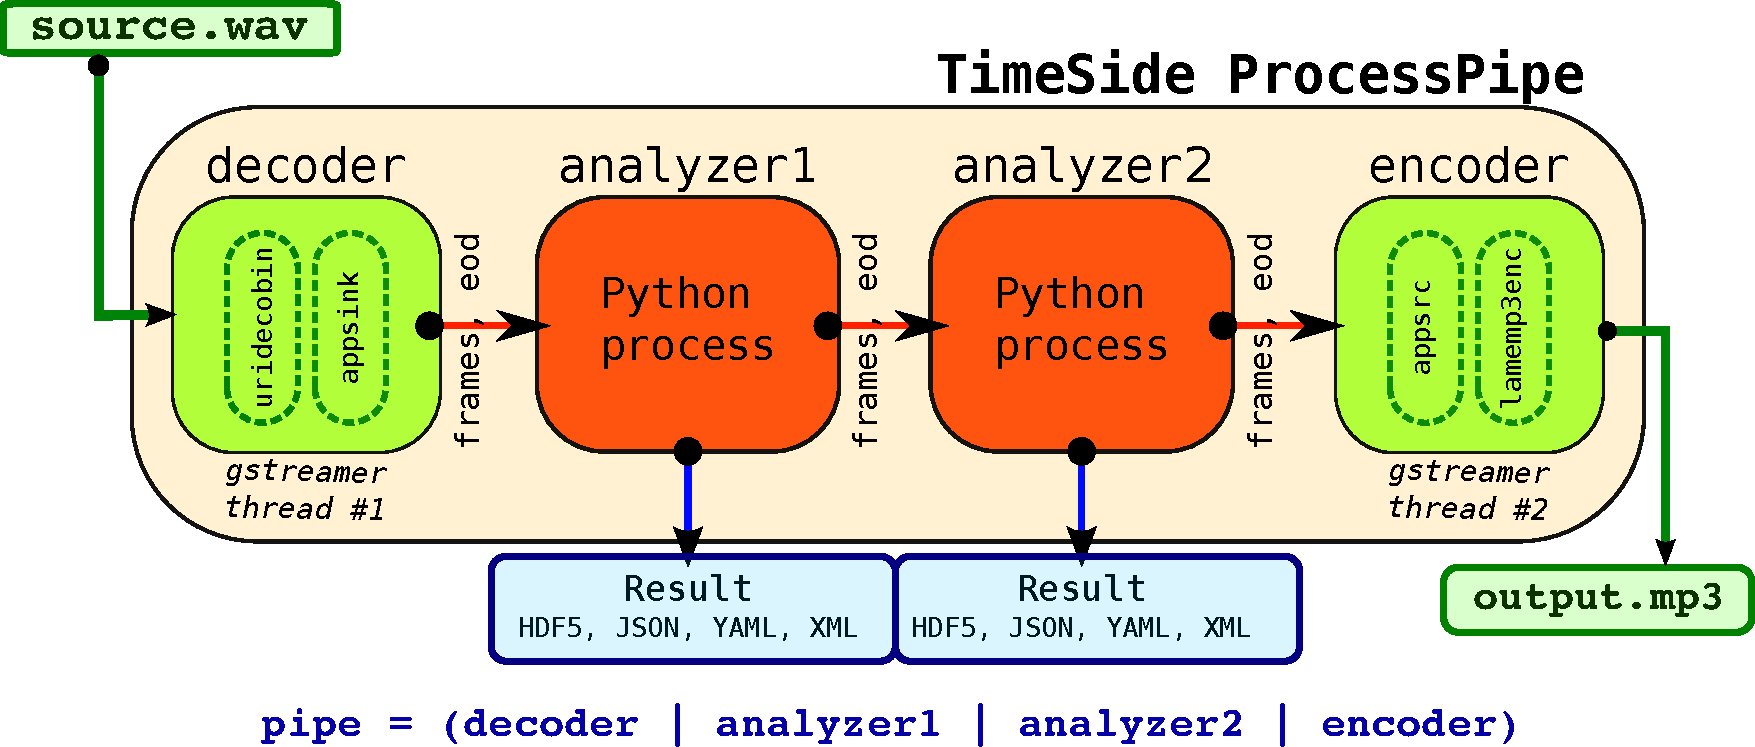
\includegraphics[width=0.95\textwidth]{img/TimeSide_pipe.pdf}
  \end{center}
  \begin{block}{Process Pipe}
    \begin{itemize}
    \item On-the-fly audio processing by simultaneous processors (decoder, encoders, analyzers, graphers)
    \item Use of \emph{Gstreamer} for audio decoding and encoding    \end{itemize}
  \end{block}
\end{frame}


\section[CNRS-MH]{Les archives sonores du CNRS - Musée de l'Homme}\label{sec:archives-CREM}
    
    \subsection{Les fonds}
   \begin{frame}\frametitle{Les fonds}
     \begin{block}{}
       \begin{itemize}
       \item One of the most important Sound archives library in Europe
       \item Most of the recordings come from the fieldwork of
      researchers in \alert{all continents} during the last \alert{110 years}.

    \item Nearly \alert{3700 hours of published record collections} e.g. more than 5000 rare discs
    \item \alert{4000 hours of unpublished recordings}, from early
      research expeditions (e.g. Dakar-Djibouti (1932), Ogooué-Congo
      (1946))
    \item \alert{47,200 items} containing more than
      \alert{26,000 sound files}, including 12,000 sounds on free
      access since May 2014
          
       \end{itemize}
     \end{block}
    \end{frame}
    
    \subsection{Usages}
     \begin{frame}\frametitle{Usages}
      \begin{block}{}
       \begin{itemize}
    \item Ethnomusicologie, Anthropologie, Linguistique, Muséologogie, Histoire de L'art
    \item Utilisateurs : chercheurs, documentalistes, professeurs, étudiants
    \item Collaborations, nouvelles pistes de recherches, "retour au pays"
    \item $\simeq2500$ utilisateurs uniques / mois
    \item 626 éditions en moyenne / semaine depuis 3 ans
       \end{itemize}
     \end{block}
     \end{frame}
     
     
    \begin{frame}{Usages}
    \begin{block}{A collaborative experience}
        \begin{itemize}
    \item The sharing of data offer resources to researchers from all over the world and allows several people to \alert{collaborate on the enrichment of the database}.
     \item Researchers from different institutions can work together on
      specific audio materials and conduct individual research from
      both synchronic and diachronic perspectives on their own
      material, the material of others, or both.
    \item Users can submit their own archives to protect them.

    \item Furthermore, it facilitates the ethical task of \alert{returning
      the recorded music to the communities who produced it} and to get local populations involved in their own cultural heritage.   
        \end{itemize}
    \end{block}

    \end{frame}

    \begin{frame}[plain, label=geonavigator]{Telemeta - Geographic Navigator}
    \begin{center}
        \fbox{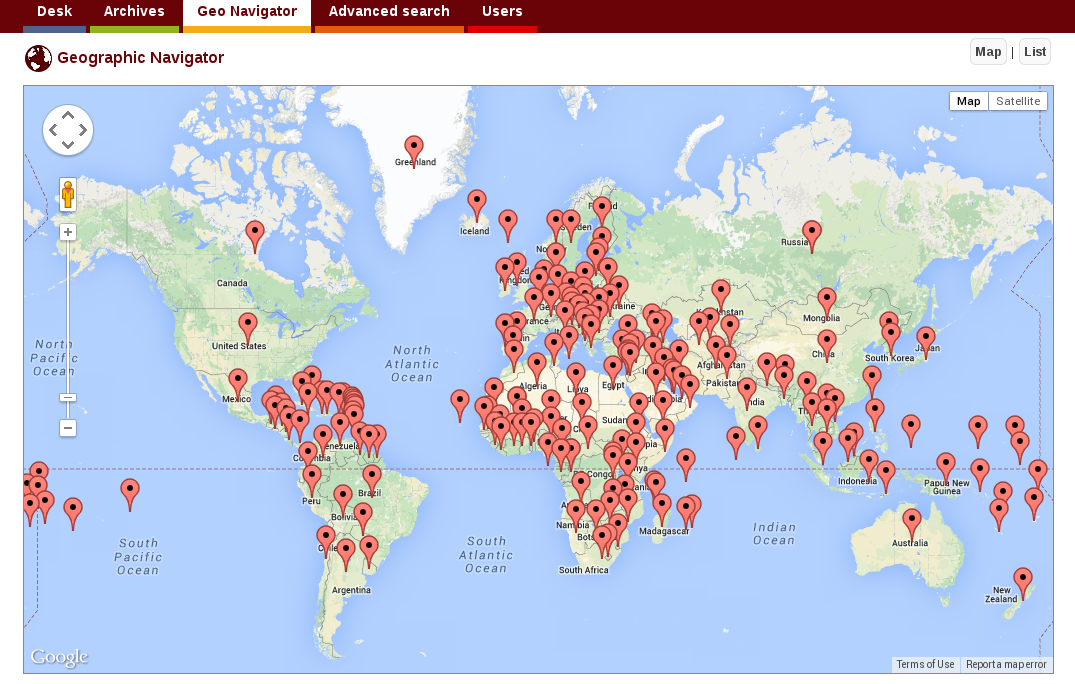
\includegraphics[width=\linewidth]{img/telemeta_geo.png}}
    \end{center}
    \hyperlink{telemeta_features}{\beamerbutton{back}}
\end{frame}

    
\section[Le projet DIADEMS]{Le projet DIADEMS}\label{sec:Diadems}

\subsection{Le consortium}

\begin{frame}{The DIADEMS project}
  \scriptsize

  Projet ANR CONTINT 2013 - 2015\\
  "Description, Indexation, Accès aux Documents Ethnomusicologiques et Sonores"
  
  \begin{block}{Le consortium}\tiny
    \begin{columns}[T]
      \begin{column}{.5\textwidth}
        \begin{block}{Science and Technology of Information and
            Communication domain}
          \begin{tabular}{p{0.27\textwidth} p{0.5\textwidth}}
            \raisebox{-0.5\height}{
\includegraphics[width=1.7cm]{img/IRIT.jpeg}} 
            &  Institute of research in computing science of Toulouse \\%[1pt]
            \raisebox{-0.7\height}{
\includegraphics[height=0.75cm]{img/LIMSI.png}} 
            & Laboratory of computing and mechanics for engineering sciences \\%[3pt]
            \raisebox{-0.6\height}{
\includegraphics[height=0.75cm]{img/LaBRI.jpeg}}
            & Bordeaux Computer Science Research Laboratory\\[5pt]
            \raisebox{-0.7\height}{
\includegraphics[height=0.65cm]{img/LAM.png}} 
            & Laboratory of Musical Acoustic, Jean Le Rond d'Alembert Institute
          \end{tabular}
        \end{block}
      \end{column}
      \begin{column}{.5\textwidth}
        \begin{block}{Musicology and Ethnomusicology domain}
          \begin{tabular}{p{0.15\textwidth} p{0.75\textwidth}}
            \raisebox{-0.5\height}{
\includegraphics[width=1.2cm]{img/LESC.png}}
            & Laboratory of Ethnology and Comparative Sociology\\[6pt]
            \raisebox{-0.5\height}{
\includegraphics[height=0.9cm]{img/logo_CREM.png}} 
            & Research Center for Ethno\-musi\-co\-logy\\[14pt]
            \raisebox{-0.5\height}{
\includegraphics[height=1.2cm]{img/MNHN.jpeg}}
            & National Museum of Natural History
          \end{tabular}
        \end{block}

      \end{column}
    
    \end{columns}
    \begin{block}{Development}
      \raisebox{-0.5\height}{\includegraphics[height=0.7cm]{img/parisson_logo_FINALE_com.pdf}}
      \hspace{0.1cm} Parisson, the company involved in the development
      of Telemeta.
    \end{block}
 
  \end{block}
\end{frame}

\subsection{Les objectifs}
\begin{frame}{Objectifs interdisciplinaires}
 
    \begin{itemize}
    \item \alert{Identification} les zones d'intérêt ethnomusicologiques et techniques (vocabulaire, grammaire, ontologies)
    \item \alert{Compréhension et définition} les liens sémio-acoustiques et spécifier les classes, les tâches d'indexation
    \item \alert{Définition} des corpus d'étude
    \item \alert{Développement} des algorithmes d'indexation semi-automatiques (modélisation, apprentissage)
    \item \alert{Implémentation} dans le moteur TimeSide
    \item \alert{Conception et intégration} des interfaces (segmentation, paramétrage, visualisation)
    \item \alert{Confrontation} les algorithmes aux aléats de la musique environnementale (bruits techniques, voix, instruments)
    \item \alert{Exploration} des méthodologies de recherche par similarités
    \end{itemize}

\end{frame}

\subsection{Les corpus}
\begin{frame}{Les corpus}
    \url{http://diadems.telemeta.org/search/corpus/?pattern=DIADEMS}
\end{frame}

\begin{frame}
\frametitle{Analyzer result examples}
\begin{center}
  \includegraphics<1>[width=\linewidth]{img/results/IRIT_Speech4Hz.png}
  \includegraphics<2>[width=\linewidth]{img/results/SOLO_DUOdetection.png}\\
  {\footnotesize \only<1>{\url{http://diadems.telemeta.org/archives/items/CNRSMH_I_2013_201_001_01/}}
  \only<2>{\url{http://diadems.telemeta.org/archives/items/CNRSMH_I_2000_008_001_04/}}}
\end{center}
\end{frame}


\section[Archivage pérenne]{Archivage pérenne}

\subsection{Problématiques}
\begin{frame}{Archivage pérenne}

  \begin{block}{Problématiques}%{Content}
    \begin{itemize}
    \item comment archiver un système de métadonnées évolutives et des données audio figées ?
    \item comment sauvegarder / cloner le système qui les lit/lie
    \item quels supports physiques ?
    \item quels protocoles et architectures ?
    \item comment éviter la sur-consommation des fermes de serveurs ?
    \end{itemize}
  \end{block}

\end{frame}

\subsection{Solutions}
\begin{frame}{Archivage pérenne}
  \begin{block}{Solutions}%{Content}
    \begin{itemize}
    \item OS libres et ouverts
    \item protocoles standards et normalisés
    \item environnements logiciels virtualisés
    \item versionnement des logiciels et des modèles de données
    \item moissonage des données au fil de l'eau (OAI-PMH, API)
    \item sauvegarde hebdomadaire des logiciels, bases de données ET logiciels sur fermes de serveurs (IN2P3 / CINES)
    \item conservation mensuelle sur NAS dédiés et "réveillés" uniquement pour la synchonisation
    \end{itemize}
  \end{block}

\end{frame}


\section{Conclusion}
% \begin{frame}\frametitle{Conclusion}
%   The Telemeta open-source framework provides a new platform for researchers in humanities and social sciences to efficiently distribute, share and work on their research on musical and sound materials. 
% This platform offers automatic music analysis capabilities through the external component, TimeSide, which provides a flexible computational analysis engine together with web serialization and visualization options. 
% The Telemeta platform provides an appropriate processing framework for researchers in computational ethnomusicology to develop and evaluate their algorithms. 
% Deployed to manage the CNRS - Musée de l’Homme sound archives, the Telemeta platform has been conceived and adapted to generate tools in line with the needs of users. 

% Thanks to the collaborative nature of the platform, users can continuously enrich metadata associated with sound archives. 
% The benefits of this collaborative platform for the field of ethnomusicology apply to numerous aspects of research, ranging from musical analysis in diachronic and synchronic comparative perspectives, as well as the long-term preservation of sound archives and the support of teaching materials for education. 

% \end{frame}


\begin{frame}{Conclusion}
  \begin{block}{}
    \begin{itemize}[<+->]
    \item Telemeta is a \alert{fully operational} web audio framework
      for managing digital sound archives 
    \item It's an \alert{open-source} software (-> feel free to use,
      fork or contribute)
    \item It's a \alert{unique collaborative multimedia platform} for digital humanities and research or education purposes.
    \item It's an \alert{wonderful development platform} for music data miners
    \end{itemize}
  \end{block}
\end{frame}

\begin{frame}{Perspectives}

  \begin{block}{Future developments}
    \begin{itemize}
    \item a smart \alert{multidimensional annotation system} (with zoom and segment selection)
    \item more \alert{social functions} (user access management and social stuff)
    \item a \alert{web API} to provide high and low level audio analysis new streaming services
    \end{itemize}
  \end{block}
\end{frame}


\subsection{Leçons}
\frame{\frametitle{Leçons}
    \begin{block}{}
    \begin{itemize}
    \item "\alert{Simplicity} is better than complexity" (\alert{KISS} principle)
    \item La \alert{modularité} est accessible avec un langage flexible (merci Python !)
    \item Les \alert{modèles} et les \alert{objets} sont plus importants que les technologies
    \item Une bonne plateforme s'appuie sur des \alert{standards}, des \alert{spécifications} et des \alert{normes}
    \item Un bon \alert{workflow} est défini par les utilisateurs (tests > feedback > revisions)
    \item Le \alert{prototypage} et le \alert{test unitaire} sont des étapes cruciales du développement.
    \item L'écosystème \alert{Open Source} international offre des possibilités immenses pour développer, collaborer,  déployer et passer les échelles d'un projet
    \end{itemize}
  \end{block}  
}


    \subsection{sponsors}
        \begin{frame}{Sponsors}


        \begin{center}
        \begin{columns}[c]
        \column{2.5cm}
        \begin{center}
            \pgfimage[width=2cm]{img/logo-ANR}
        \end{center}
        \column{2.5cm}
        \begin{center}
            \pgfimage[width=1.5cm]{img/logo-CNRS-big}
        \end{center}
        \column{2.5cm}
        \begin{center}
            \pgfimage[width=2.5cm]{img/Logo_UPX_big}
        \end{center}
        \column{2cm}
        \begin{center}
            \pgfimage[width=2cm]{img/upmc}
        \end{center}
        \end{columns}
        \end{center}

        \begin{center}
        \begin{columns}[c]
        \column{2.5cm}
        \begin{center}
            \pgfimage[width=1.5cm]{img/logo_mcc_3}
        \end{center}
        \column{2.5cm}
        \begin{center}
            \pgfimage[width=1.5cm]{img/logo-MNHN-big}
        \end{center}
        \column{2.5cm}
        \begin{center}
            \pgfimage[width=1.5cm]{img/logohumanum-web-grand-rvb}
        \end{center}
        \column{2cm}
        \begin{center}
            \pgfimage[width=2.5cm]{img/parisson_logo_200}
        \end{center}
        \end{columns}
        \end{center}

        
        \begin{center}
            \pgfimage[width=4.5cm]{img/europeana-sounds_0}
        \end{center}
        
    \end{frame}
        


\begin{frame}{Merci !}
  \begin{itemize}
  \item Contact: 
    \begin{center}\bf\href{mailto:guillaume.pellerin@parisson.com}{guillaume.pellerin@parisson.com}
     \end{center}

  \item Telemeta:
    \begin{center}
    \includegraphics[width=0.4\textwidth]{img/logo_telemeta_1-1.pdf}\\
      \textbf{\href{http://telemeta.org}{telemeta.org}}\\
      \textbf{\href{http://twitter.com/telemeta/}{@telemeta}}
    \end{center}

  \item TimeSide:
    \begin{center}
      \bf\href{https://github.com/yomguy/TimeSide/}{github.com/yomguy/TimeSide/}
    \end{center}

  \item Sound archives of the CNRS - Musée de l’Homme:
    \begin{center}
      \bf\href{http://archives.crem-cnrs.fr}{archives.crem-cnrs.fr}
    \end{center}

  \item The DIADEMS project:
    \begin{center}
      \bf\href{http://www.irit.fr/recherches/SAMOVA/DIADEMS/}{www.irit.fr/recherches/SAMOVA/DIADEMS/}
    \end{center}

  \end{itemize}
\end{frame}

\appendix
\section{Additional Materials}

\subsubsection{Multi language support}
\begin{frame}[label=telemeta_languages]{Telemeta - Multi language support}
\only<1>{\framesubtitle{English}}
\only<2>{\framesubtitle{French}}
\only<3>{\framesubtitle{German}}
\only<4>{\framesubtitle{Chinese}}

  \begin{center}
    \includegraphics<1>[width=1.1\textwidth]{img/telemeta_english.png}
    \includegraphics<2>[width=1.1\textwidth]{img/telemeta_french.png}
    \includegraphics<3>[width=1.1\textwidth]{img/telemeta_german.png}
    \includegraphics<4>[width=1.1\textwidth]{img/telemeta_chinese.png}
  \end{center}
\hyperlink{telemeta_features}{\beamerbutton{back}}
\end{frame}
\subsubsection{Metadata}
\begin{frame}[label=metadata_example]{Contextual Information example: Collection}
  \begin{center}
    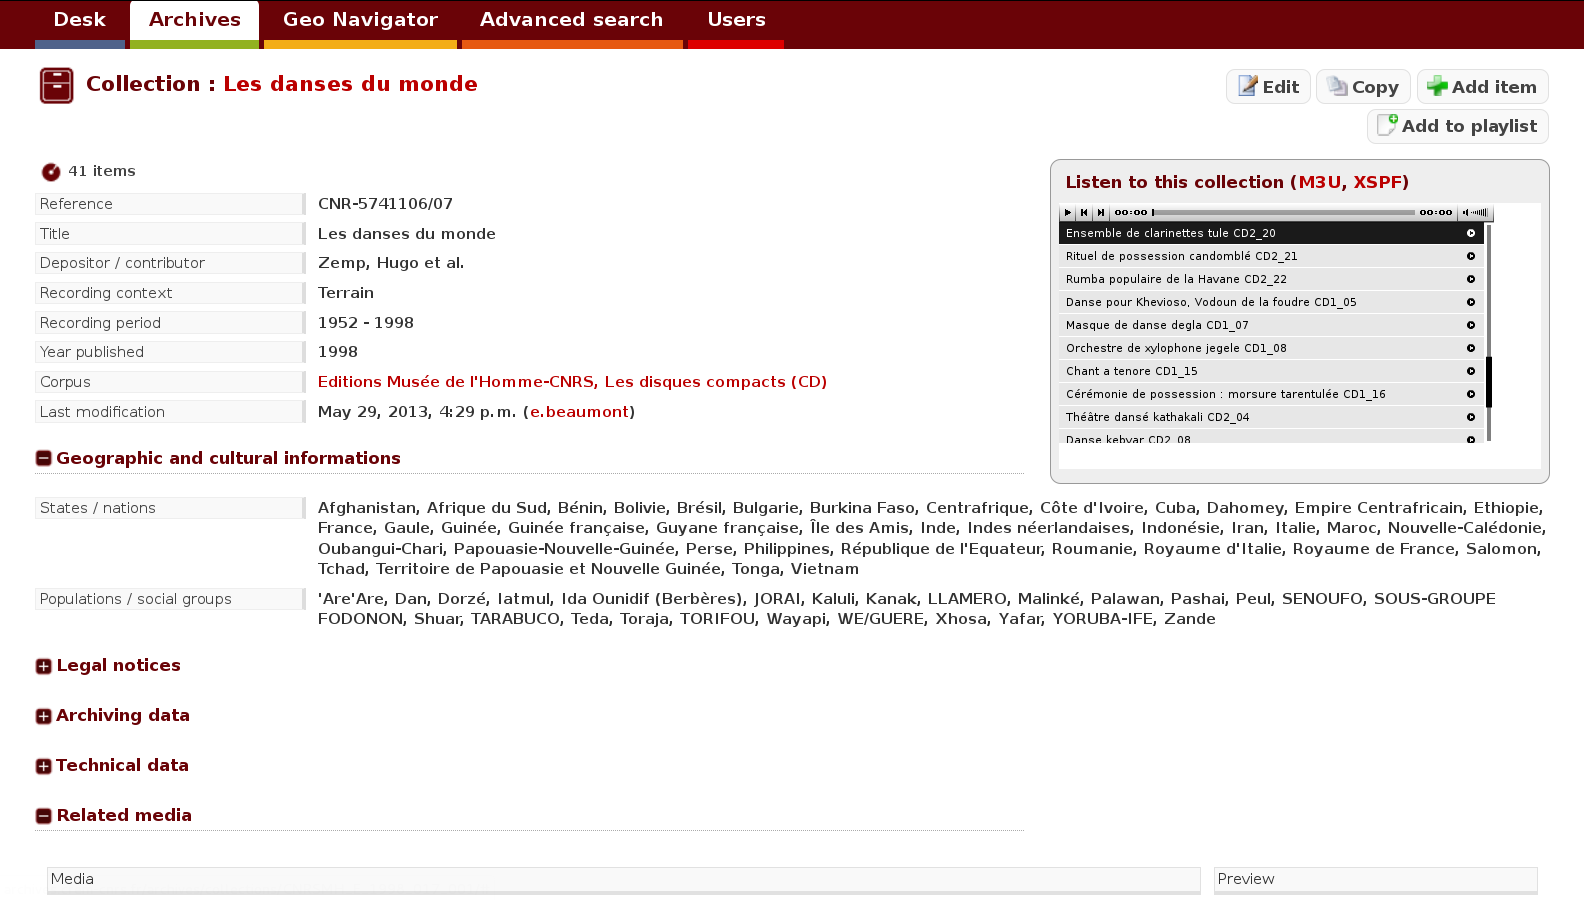
\includegraphics[width=1\textwidth]{img/telemeta_metadata_collection.png}
  \end{center}
\href{http://archives.crem-cnrs.fr/archives/collections/CNRSMH_E_1998_017_001/}{\beamerbutton{Online}}
 \href{./captures/Collection.html}{\beamerbutton{Offline}}
\hyperlink{telemeta_metadata}{\beamerbutton{back}}
\end{frame}
\begin{frame}{Contextual Information example: Item}
  \begin{center}
    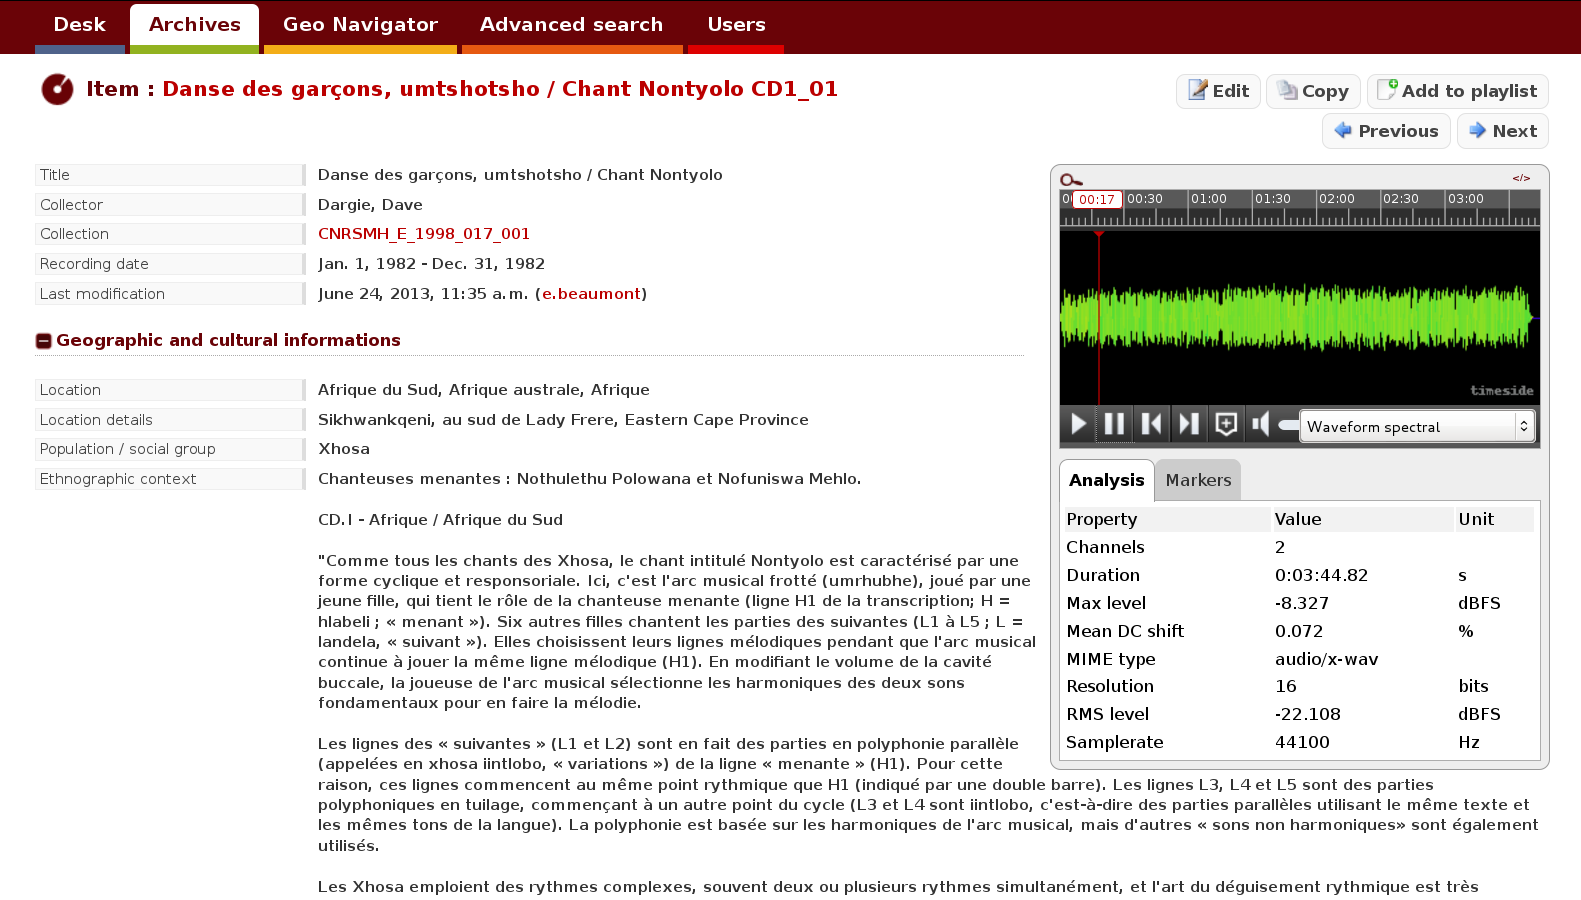
\includegraphics[width=1\textwidth]{img/telemeta_metadata_item.png}
  \end{center}
  \href{http://archives.crem-cnrs.fr/archives/items/CNRSMH_E_1998_017_001_001_01/}{\beamerbutton{Online}}
 \href{./captures/Item.html}{\beamerbutton{Offline}}
\hyperlink{telemeta_metadata}{\beamerbutton{back}}
\end{frame}
%%% Local Variables: 
%%% mode: latex
%%% TeX-master: t


\subsubsection{Supports physiques}
\begin{frame}{Supports physiques}
  \begin{block}{Etude IBM 2012}
    \begin{itemize}
    \item Tape
    \item HDD
    \item NAND
    \end{itemize}
    \end{block}

\href{http://www.digitalpreservation.gov/meetings/documents/storage12/5-Fontana-StorageMediaDenstiyfoRNANDTAPE.pdf}{\beamerbutton{PDF link}}

\begin{block}{Cas d'usage (recommandations GIS SPADON)}
    \begin{itemize}
    \item Edition (temps réel) : NAND + HDD 
    \item Sauvegarde (moyen terme) : HDD (+ NAS)
    \item Conservation (long terme) : Tape
    \end{itemize}
    \end{block}
\end{frame}

%%% End: 
\end{document}